\documentclass[10pt]{article}

\usepackage[a4paper,margin=3cm]{geometry}
\usepackage{amsmath,amsfonts,amsthm,bm}
\usepackage{amssymb}
\usepackage{afterpage}
\usepackage{lastpage}
\usepackage{graphicx}
\usepackage{fancyhdr}
\usepackage{multirow}
\usepackage{hhline}
\usepackage{titlesec}
\usepackage{enumitem}
\usepackage{mathtools}
\usepackage{indentfirst}
\usepackage{bbm}
\usepackage{float}
\usepackage[affil-it]{authblk}

\titleformat{\section}
 {\normalfont\fontsize{16}{19}\selectfont}{\thesection.}{1em}{}
\titleformat{\subsection}
 {\normalfont\fontsize{14}{17}\selectfont}{\thesubsection}{1em}{}
\titleformat{\subsubsection}
 {\normalfont\fontsize{14}{17}\selectfont}{\thesubsubsection}{1em}{}
\pagestyle{fancy}
\fancyhead{}
\fancyfoot{}
\renewcommand{\headrulewidth}{0pt}
\renewcommand{\refname}{\vskip -1cm}
\fancyfoot[R]{p. \thepage\ / \pageref{LastPage}}

\numberwithin{equation}{section}
\restylefloat{table}


\DeclareMathOperator*{\minimize}{minimize\;\;}
\DeclareMathOperator*{\subject_to}{subject\;to\;\;}
\DeclareMathOperator{\asinh}{asinh}
\DeclareMathOperator{\sgn}{sgn}


\begin{document}
\section{Project Setup}
\begin{enumerate}
    \item Project Title: A Tiny World: Atom Simulation/Rendering
    \item Members:
        \subitem Chung An, Chen (Andy), 5120AG05-1
        \subitem Yang, Liu, 5121FG59
        \subitem LinXi, Tao, 5121FG25
    \item Project Timeline:
        \subitem 12/12 - 12/15 Project Initiation (Done)
            \subsubitem Decided to go with an Atom Simulation/Rendering
            \subsubitem Backup option: Fluid simulations
        \subitem 12/15 - 12/18 Project Development Tool Investigation (Done) 
            \subsubitem Decided to use \textbf{Taichi}, a Domain-specific-language (DSL) written in Python and C++ for graphical simulations, as our main development tool
        \subitem 12/18 - 12/24 Tinkering and Experimenting with \textbf{Taichi} and Finalizing Our Initial Report
        \subitem 12/24 - 1/01 Creating Several Prototypes
        \subitem 1/01 - 1/14 Finalizing the Prototype and Refining It
        \subitem 1/14 - 1/17 Setting Up a Demo Server/Host
        \subitem 1/17 - 1/31 Creating Slides for the Presentation and Putting together Our Final Report
\end{enumerate}
\section{Project Description}
    this Project is to use \textbf{Taichi} to simulation the electron cloud.An electron cloud is a graph that uses the sparsity of small black dots to indicate the probability of occurrence of each electron in space.
    
\begin{figure}[htbp]
  \vspace{10pt} % 调整图片与上文的垂直距离
  \centering
  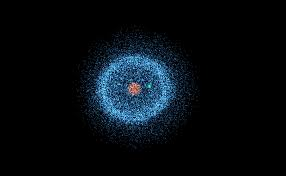
\includegraphics[]{./concept_1.jpeg}
  \caption{electron cloud}\label{fig1} % label 用来在文中索引
\end{figure}

\begin{figure}[htbp]
  \vspace{10pt} % 调整图片与上文的垂直距离
  \centering
  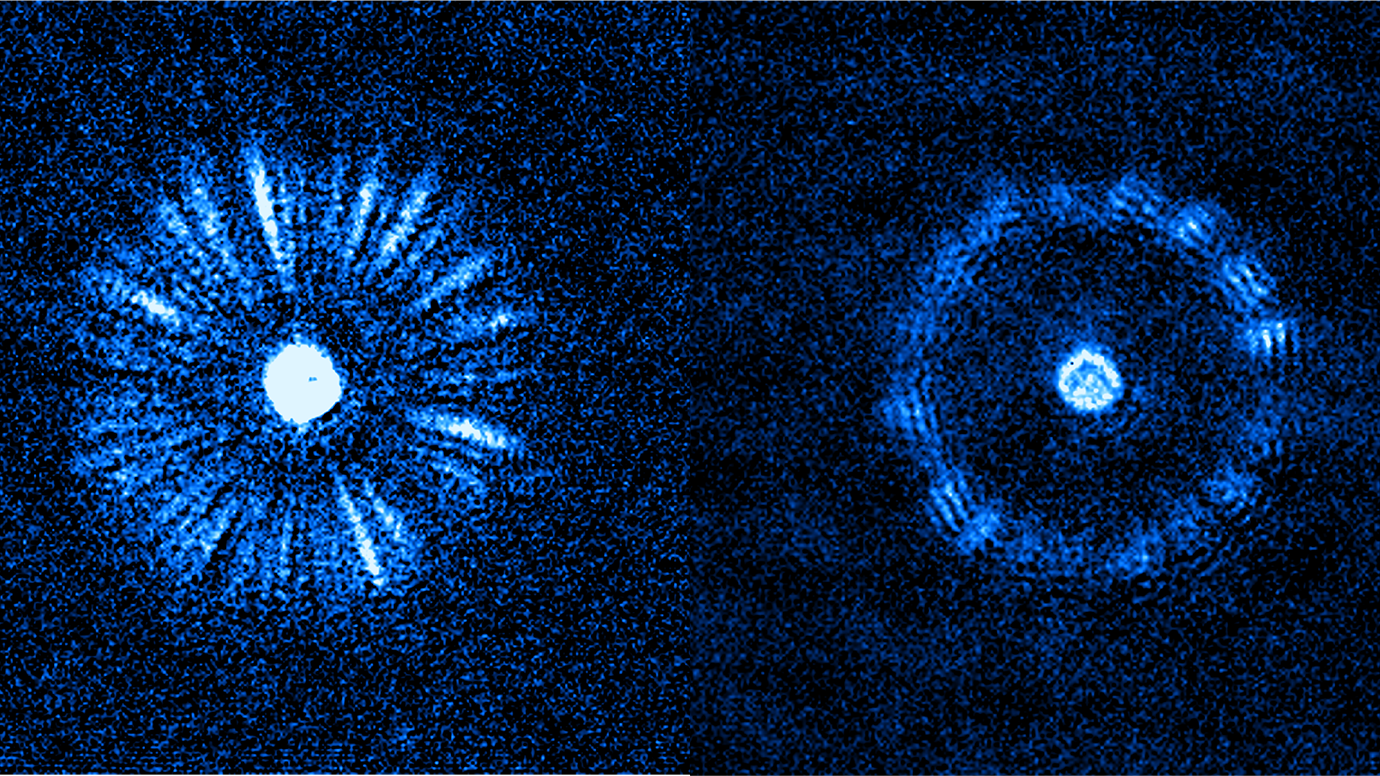
\includegraphics[]{./concept_2.png}
  \caption{electron cloud}\label{fig2} % label 用来在文中索引
\end{figure}

\section{Roles}
\begin{itemize}
    \item Chung An, Chen (Andy), 
    \item LinXi, Tao, 
    \item Yang, Liu, user interface
\end{itemize}
\end{document}
